\pagebreak % TEMP
\section{Supplemental Results}\label{app.sr.res}
Additional information on data sources, analysis, and results are available
in a public repository:\\
\hreftt{github.com/mishra-lab/sr-heterogeneity-hiv-models}
%===================================================================================================
\subsection{Map}\label{app.sr.res.map}
\begin{figure}[h]
  \centering
  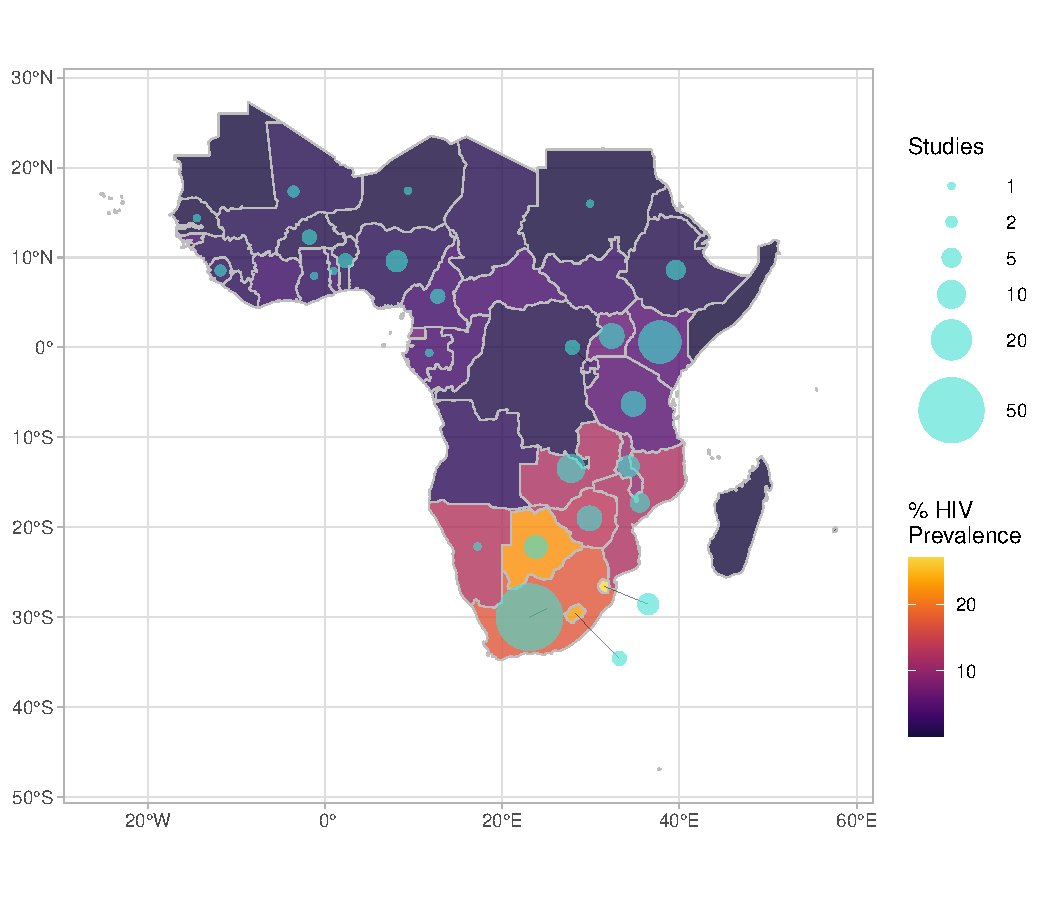
\includegraphics[width=.8\linewidth]{sr.map}
  \caption{Map showing number of studies (of 94 total)
    applying HIV transmission modelling in each country \vs
    the number of people living with HIV (PLHIV, millions)}
  \label{fig:sr.map}
\end{figure}
%===================================================================================================
\subsection{Risk Heterogeneity}\label{app.sr.res.risk}
%---------------------------------------------------------------------------------------------------
\subsubsection{Distributions}
The following figures illustrate the distributions (number of studies)
of various parameter values and modelling assumptions related to
factors of heterogeneity and intervention contexts.
\par\bigskip
\iterfig{sr.dist}{.5}{\srplotlistdist}{%
  Distributions of parameter values and modelling assumptions related to
  factors of heterogeneity and intervention contexts}{}
\pagebreak % TEMP
%===================================================================================================
\subsection{ART Prevention Impact}\label{app.sr.res.api}
The following figures illustrate the projected ART prevention impact (\srds{B}),
stratified by various factors of heterogeneity and intervention contexts (colours).
Left panels show the relative HIV incidence reduction (IR);
right panels show the proportion of cumulative HIV infections averted (CIA);
both as compared to a base-case scenario reflecting status quo.
If any study included multiple scenarios of ART scale-up,
then each scenario was included separately;
if any scenario reported multiple time horizons,
each time horizon was included separately.
The number of studies (scenarios) reporting
incidence reduction, cumulative infections averted, both, or either was:
23~(61), 24~(75), 7~(11), and 40~(125), respectively.
If any factor could not be quantified due to missing data or varying values,
it was omitted from that plot.
In box plots, the numbers of unique scenario time-horizons
contributing to each box are given above it.
\iterfig[.api]{sr}{.5}{\srplotlistapi}{%
  Projected ART prevention impacts:
  incidence reduction (IR) and cumulative infections averted (CIA),
  stratified by factors of heterogeneity and intervention contexts}{}
